%%FIG Machines
\begin{figure}[ht]
\centering
\begin{tikzpicture}[font=\small]
  \draw[thick, -{Stealth[length=2.5mm]}] (0,0) -- (15.6,0);
  \foreach \x/\d in {0/25 Jul, 1.6/2 Aug, 3.0/6 Aug, 4.3/7 Aug, 6.6/27 Sep, 8.4/1 Oct, 9.8/4 Oct, 11.3/5 Oct, 12.8/6 Oct, 14.1/7 Oct, 15.1/8 Oct}
    { \draw (\x,0.12) -- (\x,-0.12); \node[below, font=\scriptsize, rotate=40, anchor=north east] at (\x,-0.12) {\d}; }
  \draw[decorate, decoration={brace, amplitude=5pt}] (0,0.35) -- (4.3,0.35) node[midway, above=5pt, align=center, font=\footnotesize] {Part I\\FiGS install + pipeline};
  \draw[decorate, decoration={brace, amplitude=5pt}] (6.6,0.35) -- (9.8,0.35) node[midway, above=5pt, align=center, font=\footnotesize] {Part II\\Galley + SV-Net};
  \draw[decorate, decoration={brace, amplitude=5pt}] (11.3,0.35) -- (15.1,0.35) node[midway, above=5pt, align=center, font=\footnotesize] {Part III\\semantics P0--P5, variants};
  \node[font=\scriptsize, align=center, text=black!60] at (5.45,0.45) {(no commits\\in this gap)};
\end{tikzpicture}
\caption{Timeline of the work (not to scale). Laptop and SSD in July--August, intellisense05 in August, intellisense08
from late September.}
\label{fig:timeline}
\end{figure}

\begin{figure}[ht]
\centering
\begin{tikzpicture}[node distance=5mm and 6mm, font=\small,
  box/.style={draw, rounded corners=2pt, align=center, minimum height=9mm, inner sep=3pt, fill=white},
  up/.style={box, fill=gray!12}, ours/.style={box, fill=blue!8}, arr/.style={-{Stealth[length=2mm]}, thick}]
  \node[up] (fi) at (0,0) {FiGS\\(splat simulator)};
  \node[up] (sv) at (4.2,0) {SousVide\\(expert + SV-Net)};
  \node[up] (ns) at (8.6,0) {nerfstudio / gsplat\\hloc / COLMAP / acados};
  \node[ours] (inst) at (0,1.9) {\code{install\_figs.sh}\\\code{verify\_figs.sh}};
  \node[ours] (fp) at (4.2,1.9) {\code{figs\_pipeline.py}\\\code{svnet\_pipeline.py}};
  \node[ours] (sem) at (8.6,1.9) {\code{radiance\_semantics}\\\code{semantic\_pipeline.py}};
  \node[ours, minimum width=11.5cm] (gal) at (4.3,3.6) {Galley (FastAPI + React): job queue, scene \& splat, course editor, SV-Net, splat editor};
  \node[box] (br) at (4.3,5.0) {browser (laptop, via SSH tunnel)};
  \draw[arr] (br) -- (gal); \draw[arr] (gal) -- (inst); \draw[arr] (gal) -- (fp); \draw[arr] (gal) -- (sem);
  \draw[arr] (inst) -- (fi); \draw[arr] (fp) -- (sv); \draw[arr] (fp) -- (fi); \draw[arr] (sem) -- (ns);
  \node[font=\footnotesize, text=black!60, align=left, anchor=west] at (10.8,0) {upstream, unchanged};
  \node[font=\footnotesize, text=black!60, align=left, anchor=west] at (10.8,1.9) {ours};
\end{tikzpicture}
\caption{What was built around the upstream code. Grey: upstream (pinned, unchanged); blue: this project.}
\label{fig:layers}
\end{figure}

%%FIG 5. One resumable pipeline script
\begin{figure}[ht]
\centering
\begin{tikzpicture}[font=\scriptsize, node distance=1.1mm,
  s/.style={draw, rounded corners=1.5pt, fill=orange!10, minimum height=6mm, inner sep=2pt},
  g/.style={s, fill=red!12}]
  \node[s] (a) {preflight}; \node[s, right=of a] (b) {probe}; \node[s, right=of b] (c) {transcode};
  \node[s, right=of c] (d) {aruco}; \node[s, right=of d] (e) {config}; \node[s, right=of e] (f) {patch};
  \node[g, right=of f] (g1) {sfm}; \node[g, right=of g1] (g2) {train};
  \node[s, below=4mm of a, anchor=north west, xshift=-4mm] (h) {verify}; \node[s, right=of h] (i) {bounds};
  \node[s, right=of i] (j) {course}; \node[g, right=of j] (k) {simulate}; \node[s, right=of k] (l) {validate};
  \node[s, right=of l] (m) {record};
  \foreach \u/\v in {a/b,b/c,c/d,d/e,e/f,f/g1,g1/g2,h/i,i/j,j/k,k/l,l/m} \draw[-{Stealth[length=1.3mm]}] (\u) -- (\v);
  \draw[-{Stealth[length=1.3mm]}] (g2.south) |- ($(h.north)+(0,0.2)$) -- (h.north);
\end{tikzpicture}
\caption{The pipeline's steps (the \code{gsplat} step was split into \code{sfm} + \code{train} on 27 Sep). Red: GPU
steps. Each step leaves a marker with a fingerprint of its inputs, so a re-run resumes after the last finished step.}
\end{figure}

%%FIG 6. Galley phases
\begin{figure}[ht]
\centering
\begin{tikzpicture}[font=\small, node distance=5mm and 7mm,
  box/.style={draw, rounded corners=2pt, align=center, minimum height=9mm, inner sep=3pt, fill=white},
  arr/.style={-{Stealth[length=2mm]}, thick}]
  \node[box, fill=gray!10] (br) at (0,0) {browser\\React, three.js};
  \node[box] (api) at (4.7,0) {FastAPI\\REST + WebSocket};
  \node[box] (q) at (9.6,0) {job queue of one\\SQLite: jobs, logs};
  \node[box, text width=4.4cm] (w) at (9.6,-1.9) {\code{bash -c 'source figs\_env.sh \&\& exec <script> \dots'}\\own process group};
  \node[box, fill=gray!10] (st) at (4.7,-1.9) {configs, \code{gsplats/}, \code{runs/},\\step markers, logs};
  \node[box] (tools) at (0,-1.9) {\code{course\_tools.py},\\query worker (CPU)};
  \draw[arr, <->] (br) -- node[above, font=\scriptsize] {:8800} (api);
  \draw[arr] (api) -- (q); \draw[arr] (q) -- (w); \draw[arr] (w) -- (st); \draw[arr] (api) -- (st);
  \draw[arr] (api) -- (tools);
\end{tikzpicture}
\caption{Galley's architecture. The scripts remain the source of truth: Galley builds validated argument lists, runs one
GPU job at a time, and reads the scripts' state files.}
\end{figure}

%%FIG Part III
\begin{figure}[ht]
\centering
\begin{tikzpicture}[font=\small, node distance=4mm and 5mm,
  p/.style={draw, rounded corners=2pt, align=center, minimum height=11mm, text width=2.15cm, inner sep=2pt},
  arr/.style={-{Stealth[length=2mm]}, thick}]
  \node[p, fill=green!15] (p0) {P0 env + poses\\\scriptsize 5 Oct};
  \node[p, fill=green!15, right=of p0] (p1) {P1 lift + query\\\scriptsize 5 Oct};
  \node[p, fill=green!15, right=of p1] (p2) {P2 Galley API\\\scriptsize 5 Oct};
  \node[p, fill=green!15, right=of p2] (p3) {P3 splat editor\\\scriptsize 5 Oct};
  \node[p, fill=green!15, below=of p2] (p4) {P4 FMGS\\\scriptsize 5--6 Oct};
  \node[p, fill=green!15, right=of p4] (p5) {P5 evaluation\\\scriptsize 6--8 Oct};
  \node[p, fill=gray!10, right=of p5] (p6) {P6 instructions\\\scriptsize not started};
  \draw[arr] (p0) -- (p1); \draw[arr] (p1) -- (p2); \draw[arr] (p2) -- (p3);
  \draw[arr] (p1) |- (p4); \draw[arr] (p3) -- (p5); \draw[arr] (p4) -- (p5); \draw[arr] (p5) -- (p6);
\end{tikzpicture}
\caption{The semantics phases and their gates (green: passed).}
\end{figure}

\begin{figure}[ht]
\centering
\begin{tikzpicture}[node distance=4mm and 5mm, font=\small,
  box/.style={draw, rounded corners=2pt, align=center, minimum height=8mm, inner sep=3pt, fill=white},
  arr/.style={-{Stealth[length=2mm]}, thick}]
  \node[box, fill=gray!12] (sp) {frozen splat\\+ photos};
  \node[box, right=of sp] (t) {teachers\\CLIP, DINOv2};
  \node[box, right=of t, yshift=7mm] (l) {lift};
  \node[box, right=of t, yshift=-7mm] (f) {FMGS};
  \node[box, fill=gray!12, right=of l, yshift=-7mm] (tab) {per-Gaussian\\table};
  \node[box, right=of tab] (q) {query\\(CPU worker)};
  \node[box, right=of q] (c) {goal $\rightarrow$\\course $\rightarrow$ flight};
  \draw[arr] (sp) -- (t); \draw[arr] (t) -- (l); \draw[arr] (t) -- (f); \draw[arr] (l) -- (tab); \draw[arr] (f) -- (tab);
  \draw[arr] (tab) -- (q); \draw[arr] (q) -- (c);
\end{tikzpicture}
\caption{The semantic layer in one line (details in \code{semantic\_embedding\_report.pdf}).}
\end{figure}

%%FIG 13. Phase 4
\begin{figure}[ht]
\centering
\begin{tikzpicture}[font=\small, node distance=4mm and 4mm,
  r/.style={draw, rounded corners=2pt, align=center, minimum height=12mm, text width=2.4cm, inner sep=2pt},
  arr/.style={-{Stealth[length=2mm]}, thick}]
  \node[r, fill=red!12] (r1) {run 1: tcnn will not\\launch a 192-d grid};
  \node[r, fill=red!12, right=of r1] (r2) {run 2: tcnn OOM\\(two allocators)};
  \node[r, fill=red!12, right=of r2] (r3) {debug: NaN at step 11\\(fp16 under/overflow)};
  \node[r, fill=green!15, right=of r3] (r4) {run 3: PASSED\\31.4 min, 7.95 GB};
  \node[r, below=of r1, fill=blue!6] (x1) {split grid\\$2\times12$ levels};
  \node[r, below=of r2, fill=blue!6] (x2) {expandable segments,\\OOM retry};
  \node[r, below=of r3, fill=blue!6] (x3) {GradScaler,\\norm floor};
  \draw[arr] (r1) -- (r2); \draw[arr] (r2) -- (r3); \draw[arr] (r3) -- (r4);
  \draw[arr, dashed] (r1) -- (x1); \draw[arr, dashed] (r2) -- (x2); \draw[arr, dashed] (r3) -- (x3);
\end{tikzpicture}
\caption{The Phase 4 gate: three failures, each with its fix, before the pass.}
\end{figure}

%%FIG 17. Improving B and C
\begin{figure}[ht]
\centering
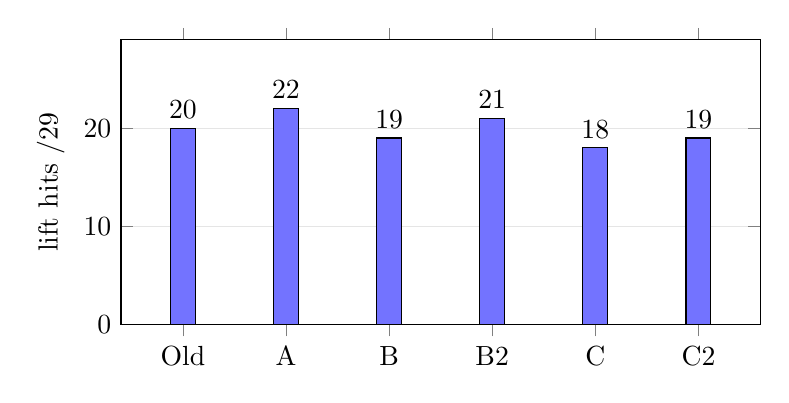
\begin{tikzpicture}
\begin{axis}[ybar, bar width=9pt, width=0.8\linewidth, height=5.2cm, ymin=0, ymax=29, ylabel={lift hits /29},
  symbolic x coords={Old,A,B,B2,C,C2}, xtick=data, nodes near coords, ymajorgrids, grid style={gray!20},
  enlarge x limits=0.12]
  \addplot[fill=blue!55] coordinates {(Old,20) (A,22) (B,19) (B2,21) (C,18) (C2,19)};
\end{axis}
\end{tikzpicture}
\caption{Lift (L-C) hits per teacher design at the default floor, amended query sets. With a floor sweep, B2 without
level choice reaches 24/29 at the same false-positive count.}
\end{figure}
